%!TEX root = ../iceDetection.tex

\documentclass[a4paper,14pt]{extarticle}

\usepackage{cmap}
\usepackage[T2A]{fontenc}
\usepackage[utf8x]{inputenc}
% \usepackage{mathptmx}
\usepackage[english, russian]{babel}

\usepackage{misccorr}
\usepackage{amssymb,amsfonts,amsmath,amsthm}  
\usepackage{indentfirst}
\usepackage[usenames,dvipsnames]{color} 
\usepackage[unicode,hidelinks]{hyperref}
\usepackage{makecell,multirow} 
\usepackage{ulem}
\usepackage{graphicx,wrapfig}
\graphicspath{{img/}}

\renewcommand{\labelenumii}{\theenumii)} 
\newcommand{\mean}[1]{\langle#1\rangle}

\DeclareMathOperator{\Div}{div}
\DeclareMathOperator{\const}{const}
%%%%%%%%%%%%%%%%%%%%%%%%%%%%%%%%%%%%%%%%%%%%%%%%%%%%%%%%%%%%%%%%%%%%%%%%%%%%%%%
%%%%%%%%%%%%%%%%%%%%%%%%%%%%%%%%%%%%%%%%%%%%%%%%%%%%%%%%%%%%%%%%%%%%%%%%%%%%%%%
\usepackage{float}
\usepackage[mode=buildnew]{standalone}
\usepackage[outline]{contour}
\usepackage{tocloft}
\renewcommand{\cftsecleader}{\cftdotfill{\cftdotsep}} % for parts
% \renewcommand{\cftchapleader}{\cftdotfill{\cftdotsep}} % for chapters
\usepackage{pgfplots,pgfplotstable,booktabs,colortbl}
\usepackage{physics}
\usepackage{mathtools}
% \mathtoolsset{showonlyrefs=true}

% \newcommand*\dotvec[1][1,1]{\crossproducttemp#1\relax}
% \def\crossproducttemp#1,#2\relax{{\qty[\vec{#1}\times\vec{#2}\,]}}

% \newcommand*\prodvec[1][1,1]{\crossproducttempa#1\relax}
% \def\crossproducttempa#1,#2\relax{{\qty[{#1}\times{#2}\,]}}
% \usepackage{showframe}
\usepackage[]{geometry}
\geometry{
  left=2.5cm,
  right=1.5cm,
  top=2cm,
  bottom=2cm,
  bindingoffset=0cm,
  headheight=17pt
}
\linespread{1.5} 
\setlength{\parindent}{1.25cm}
\frenchspacing 
\usepackage{setspace}
\setlength{\tabcolsep}{20pt}
\renewcommand{\arraystretch}{1.5}
\usepackage{xcolor}



\begin{document}

%!TEX root = ../iceDetection.tex
\begin{titlepage}
	\begin{center}
	  {\fontsize{ 12pt }{ 12pt } \selectfont \bf 
	  МИНИСТЕРСТВО НАУКИ И ВЫСШЕГО ОБРАЗОВАНИЯ \\[-10pt] 
	  РОССИЙСКОЙ ФЕДЕРАЦИИ}\\
	  \vspace{12pt}
	  \begin{spacing}{1}
		{\bf  Федеральное государственное автономное \\
		образовательное учреждение высшего образования \\
		<<Национальный исследовательский \\ 
		Нижегородский государственный университет им. Н.И. Лобачевского>>
		}
	  \end{spacing}
	  \vspace{24pt}
	  \begin{spacing}{1}
		Радиофизический факультет\\
		Кафедра общей физики\\
		\vspace{20pt}
		Направление <<Радиофизика>>\\
		\vspace{20pt}
		{ \fontsize{18pt}{18pt}ОТЧЕТ ПО УЧЕБНОЙ ПРАКТИКЕ}\\
		(Практика по получению первичных профессиональных умений и навыков, в том числе первичных умений и навыков научно-исследовательской деятельности\\
		% \vspace{20pt}
		% { \fontsize{18pt}{18pt} \bf Детектирование ледяного покрова по данным двухчастотного радиолокатора}
	  \end{spacing}
	  \vspace{100pt}
	  
		\begin{align*}
		  &\text{Руководитель практики:}\quad &\text{Панфилова М.\,А.}\\
		  &\text{Студент 3-го курса бакалавриата:}\quad &\text{Шиков А.\,П.}
		\end{align*}
	 
	\end{center}
	\vfill
	\begin{center}
	  {Нижний Новгород, 2019}
	\end{center}
  \end{titlepage}



\tableofcontents
\newpage
\section{Введение}
% \addcontentsline{toc}{section}{Введение}

Мониторинг ледяного покрова является важной задачей для решения как научных, так и практических проблем. Он широко
применяется в мореходстве, предсказании изменений климата и погоды, а также для решения различных фундаментальных задач.
Спутниковое наблюдение обладает огромными возможностями в реализации мониторинга интересующих областей.
Это может быть наблюдение в оптическом диапазоне: в ясную погоду лед хорошо виден на оптических снимках, однако во время
облачности этот способ по понятным причинам не подходит. Помимо оптики используются данные радиометрии (пассивный
метод), а также данные радаров с синтезированной апертурой и альтиметров (активная радиолокация). Радары с
синтезированной апертурой работают в СВЧ-диапазоне при средних углах падения (20$^{\circ}$ - 60$^{\circ}$), альтиметры - при нулевом
угле падения. Исследованиями по наблюдению льда практически не охвачен диапазон малых углов падения.

В данной работе приведено исследование методов детектирования льда на поверхности моря по данным для малых углов падения
от 0$^{\circ}$ до 18$^{\circ}$ по данным двухчастотного радиолокатора, установленного на спутнике GPM (Global
Precipitation Measurment).

% \vspace{15pt}
\section{Миссия GPM}

Спутник миссии Global Precipitation Measurment \cite{skof} был запущен в феврале 2014 для обнаружения атмосферных осадков.
Он оборудован микроволновым формирователем изображений (GMI, радиометр), а также двухчастотным радаром (Dual frequency
Precipitation Radar - DPR). 

Радар работает в Ku-диапазоне (частота 13.6 ГГц, длина волны 22 мм) и Ka-диапазоне (частота 35.5 ГГц,
длина волны 8 мм). Сканирование производится перпендикулярно направлению
полета, с максимальным отклонением до 18° у Ku- диапазона, и до 9.5° у Ka-диапазона. В таблице \ref{tab:1} приведена некоторая
техническая информация о радаре. Ширина полосы обзора составляет 245 км для Ku-диапазона, 145 км для Ka-диапазона, со
средним разрешением 5 км для данных за 2014-2017 годы. Начиная с 2018 года полосы обзора для обоих диапазонов совпадают
для двух частот, их ширина 245 км. В нашей работе используются данные Ku-диапазона за 2016-2017 год.  

В ходе нескольких исследований (\cite{chu,fre,kar1,masha}), было показано, что двухчастотный радар
чувствителен не только к осадкам, но и к типу отражающей поверхности. В частности, в \cite{kar1} описывалось отличие
отраженного сигнала от поверхности воды и от поверхности льда.


\section{Рассеяние электромагнитных волн шероховатой поверхностью}

\subsection{Удельная эффективная площадь рассеяния} 

Важной характеристикой сосредоточенной цели в радиолокации является \textit{эффективная площадь рассеяния}
(ЭПР)\cite{meln}. Она выражается через плотность потока мощности падающей волны вблизи цели $\Pi_1$ и плотность потока
мощности отраженной волны, принятой РЛС $\Pi_2$
\begin{equation}
  \sigma = 4 \pi R^2 \frac{\Pi_2}{\Pi_1} = 4 \pi R^2 \frac{|E_2|^2}{|E_1|^2},
  \label{eq:1.1}
\end{equation}
где R - расстояние от РЛС до цели, $E_{1,2}$ - напряженность электрического поля вблизи цели и вблизи РЛС соответственно
(можно заменить электрические составляющие поля магнитными). Множитель $4 \pi R^2$  исключает зависимость отношения
плотностей потока от расстояния. ЭПР сильно зависит от формы, ориентации и материала облучаемого объекта. 
Поверхность Земли - распределенная цель. В этом случае имеет смысл говорить об удельной эффективной площади рассеяния
(УЭПР), обозначим ее $\sigma^0$. УЭПР равна ЭПР, нормированной на эффективную площадь засветки (см. рис. \ref{fig:1}):
\begin{equation}
  \sigma^0 = 4 \pi R^2 \frac{\Pi_2}{S\Pi_1}.
  \label{eq:1.2}
\end{equation}

\begin{figure}[h!]
  \centering
  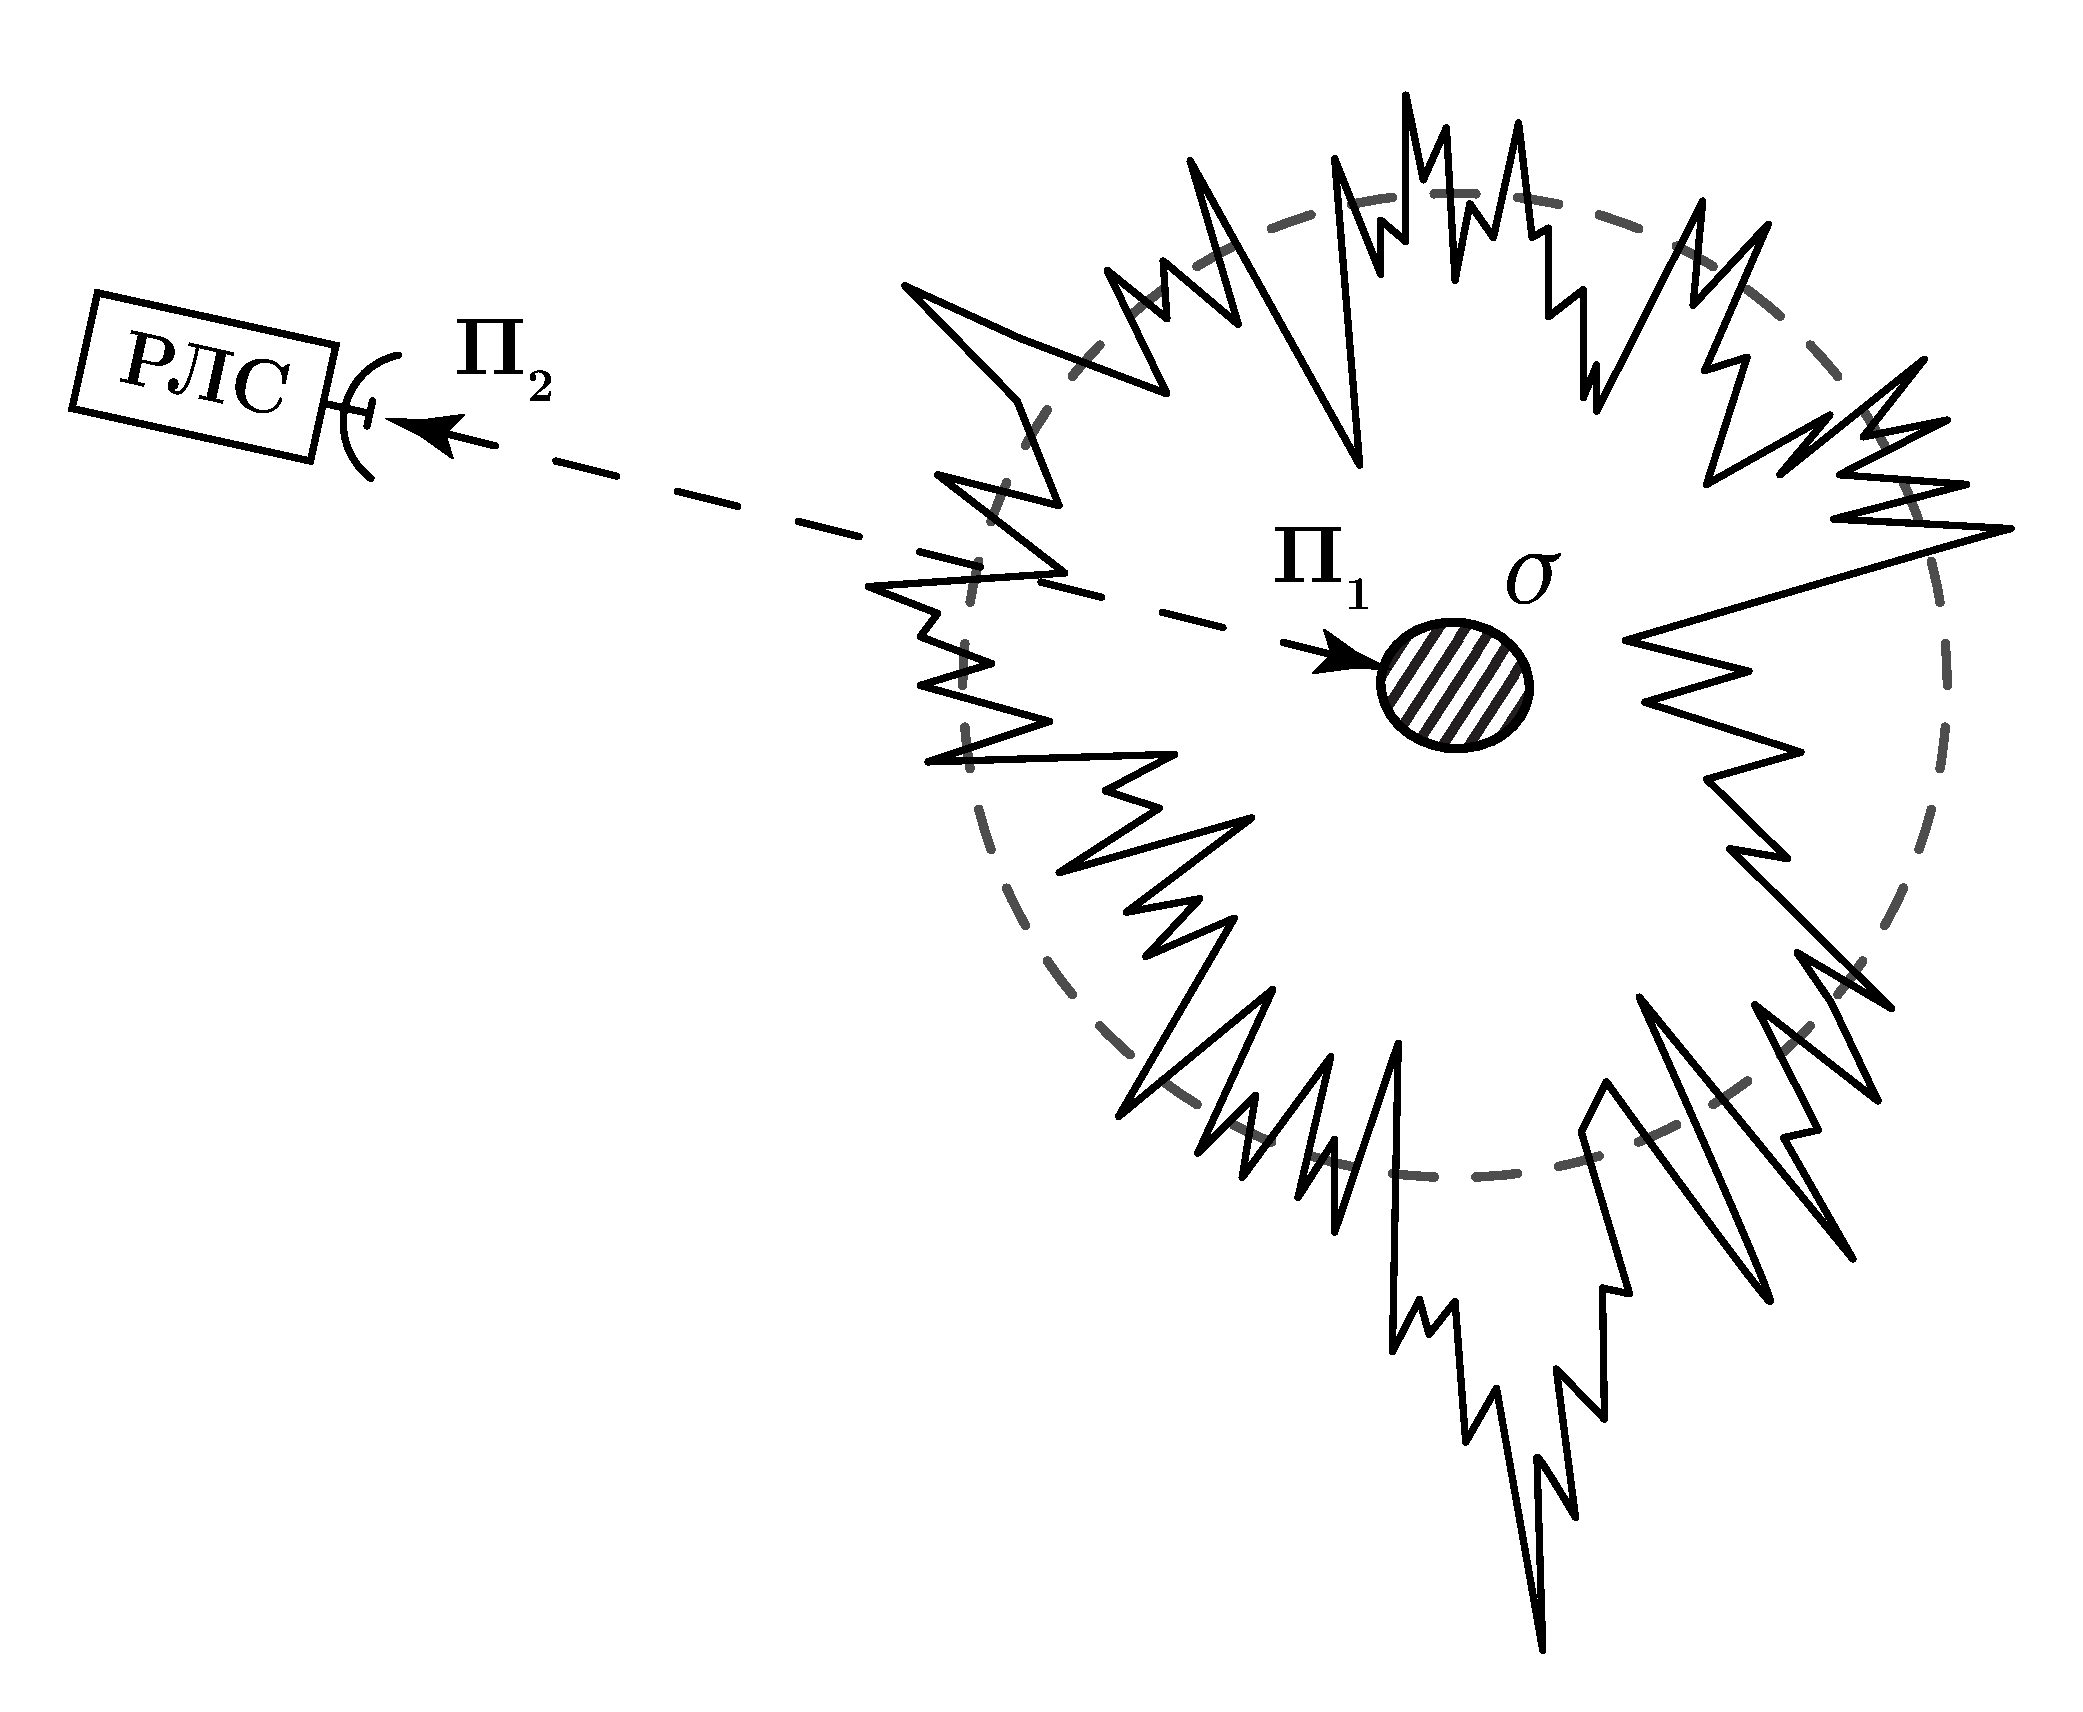
\includegraphics[width = .49\linewidth]{img/rls.pdf}
  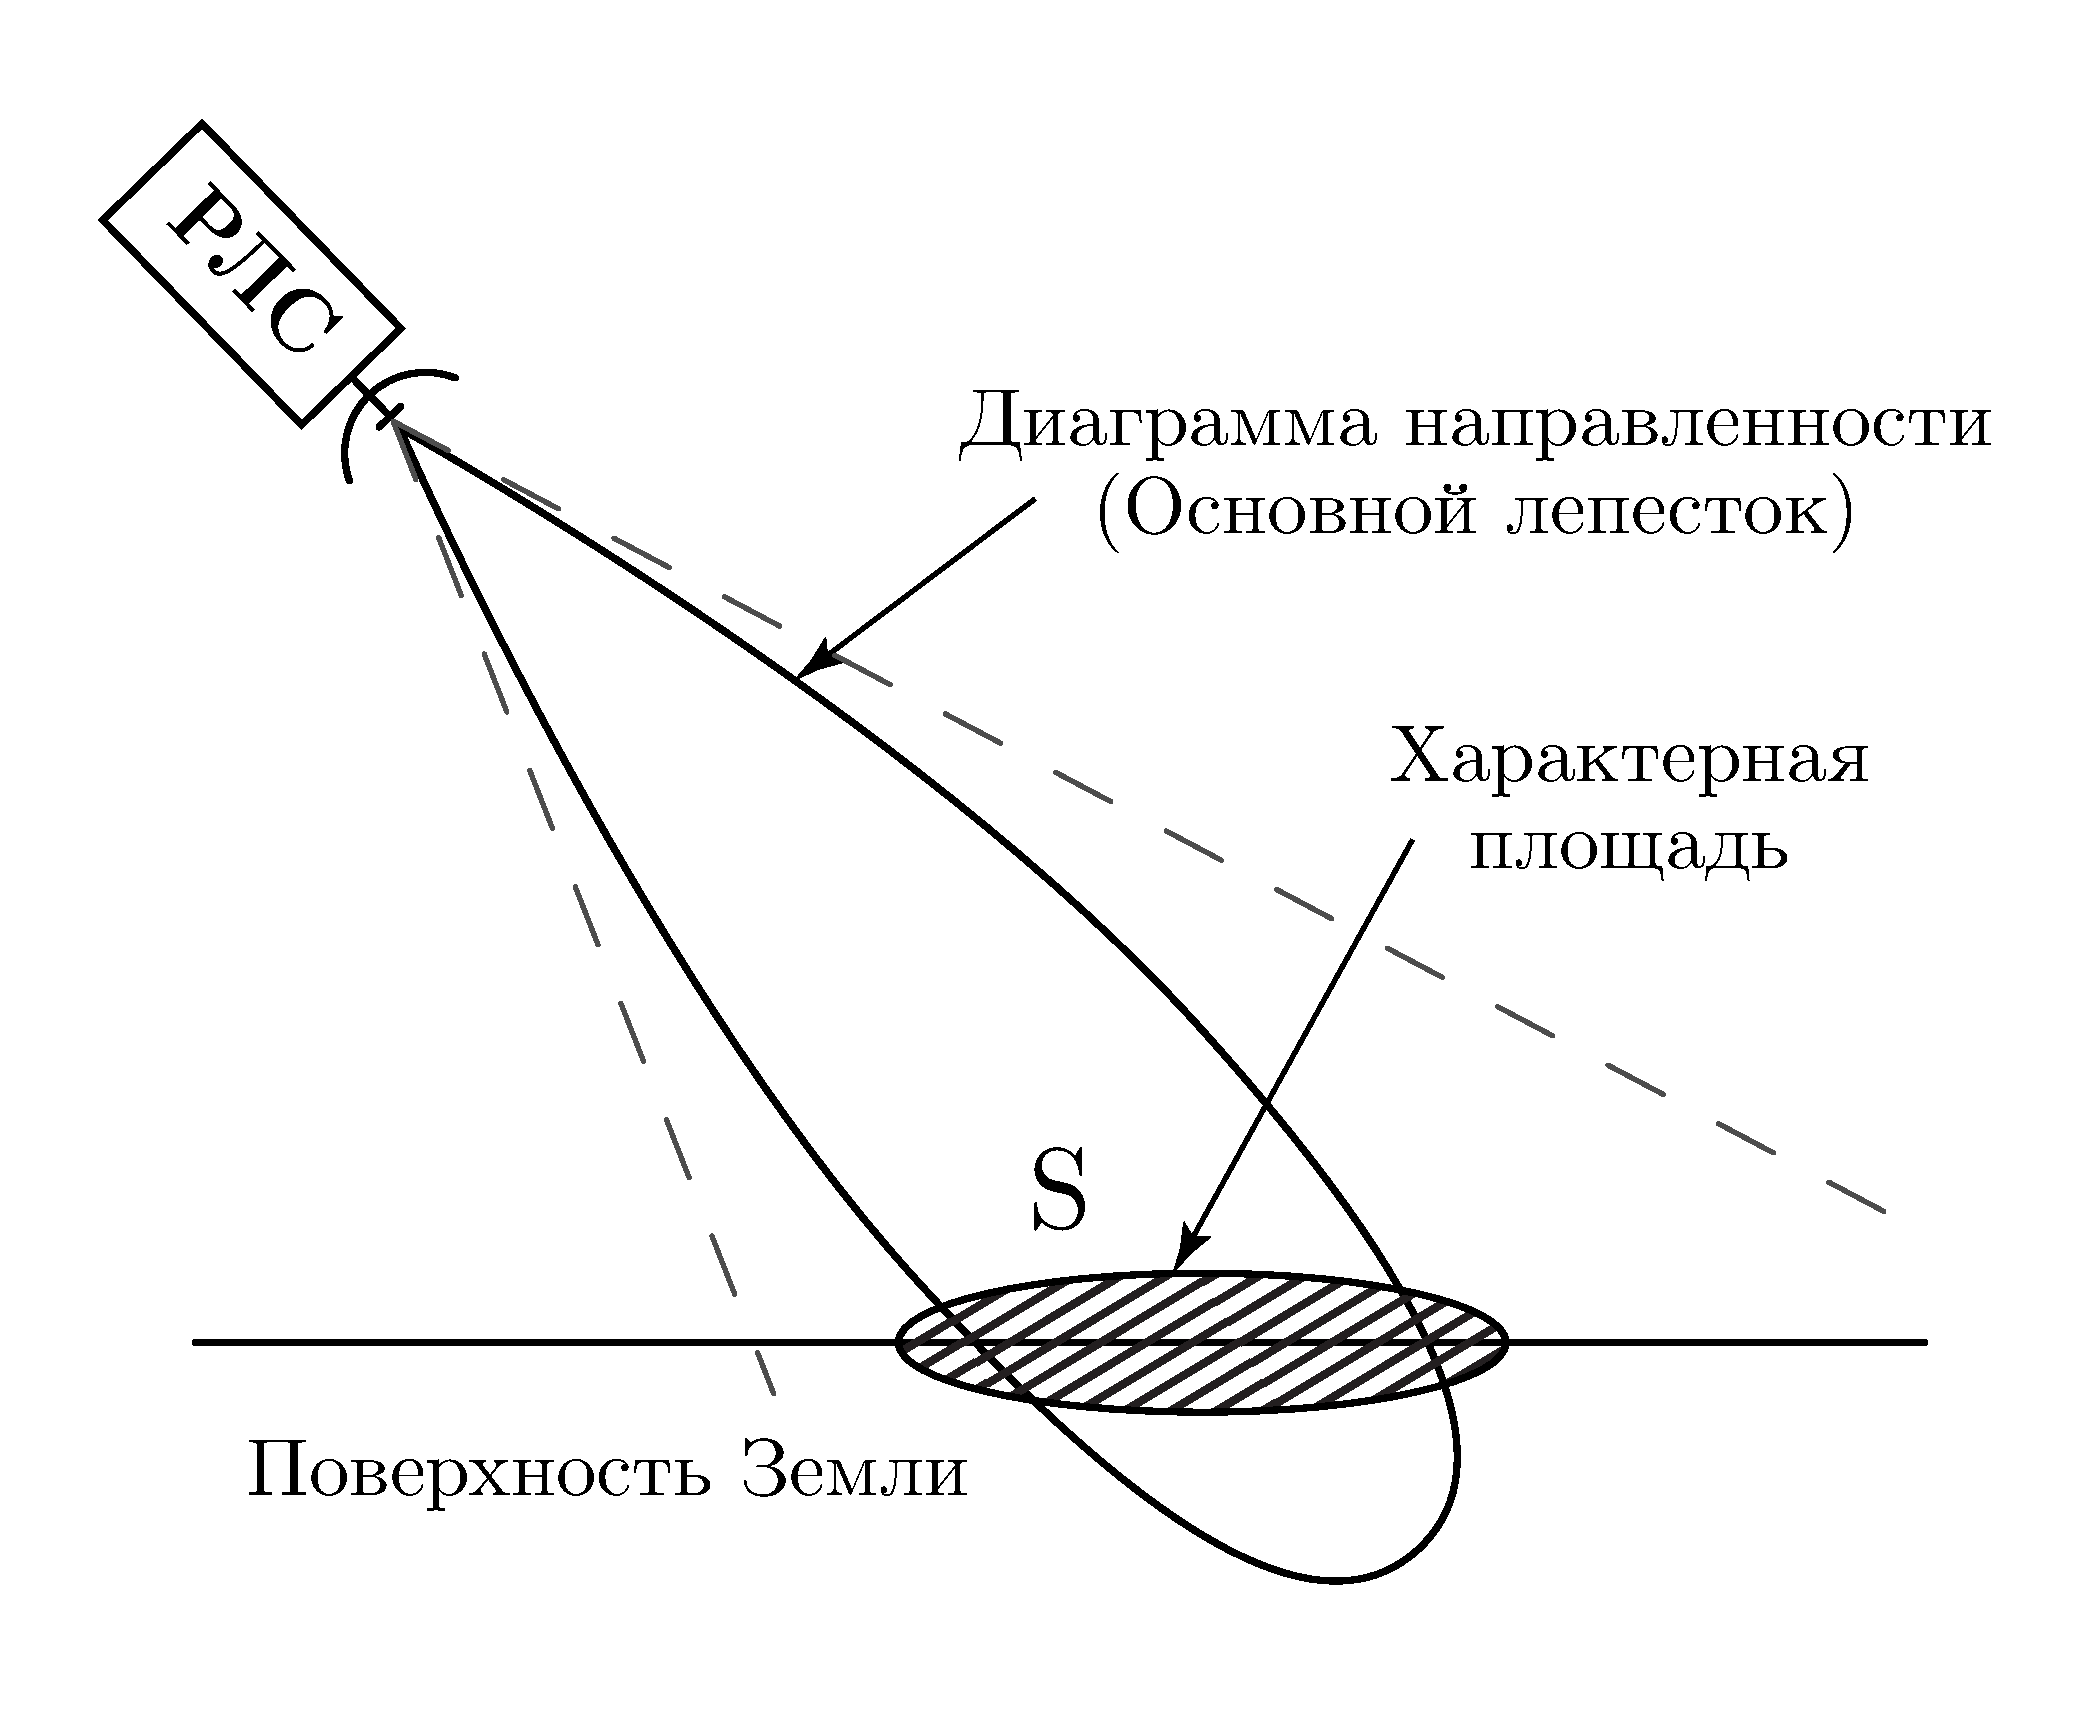
\includegraphics[width = .49\linewidth]{img/rls2.pdf}
  \caption{К формулам \eqref{eq:1.1} и \eqref{eq:1.2}. Слева - случай сосредоточенной цели, справа - распределенной цели.}
  \label{fig:1}
\end{figure}

\subsection{Случай морской поверхности}

Определения УЭПР морской поверхности  - сложная задача. Она сводится к поиску отраженного поля не для
конкретной поверхности, а параметров усредненного поля для статистического ансамбля реализаций поверхности. Для решения задачи
разработан ряд приближенных методов~\cite{bassfuks}.

Для удобства описания рассеяния СВЧ-волн морской поверхностью выделяют два характерных масштаба волнения: крупные волны,
покрытые рябью. Граница, разделяющая эти масштабы в спектре волнения, зависит от длины волны зондирующего излучения.
При зондировании под малыми углами падения зависимость УЭПР для поверхности воды от угла падения может быть описана в
рамках квазизеркального приближения. Крупномасштабная поверхность разбивается на
фасеты, и в отраженный сигнал вклад вносит излучение, отраженное только от площадок, расположенных
перпендикулярно к вектору падающей волны, а рябь влияет только на коэффициент отражнения от них, что учтено в коэффициенте $A$ в уравнении \eqref{eq:3}.
Это приближение применимо, если локальный радиус кривизны крупномасштабной поверхности много больше
длины зондирующего излучения.


\begin{figure}[h!]
  \centering
  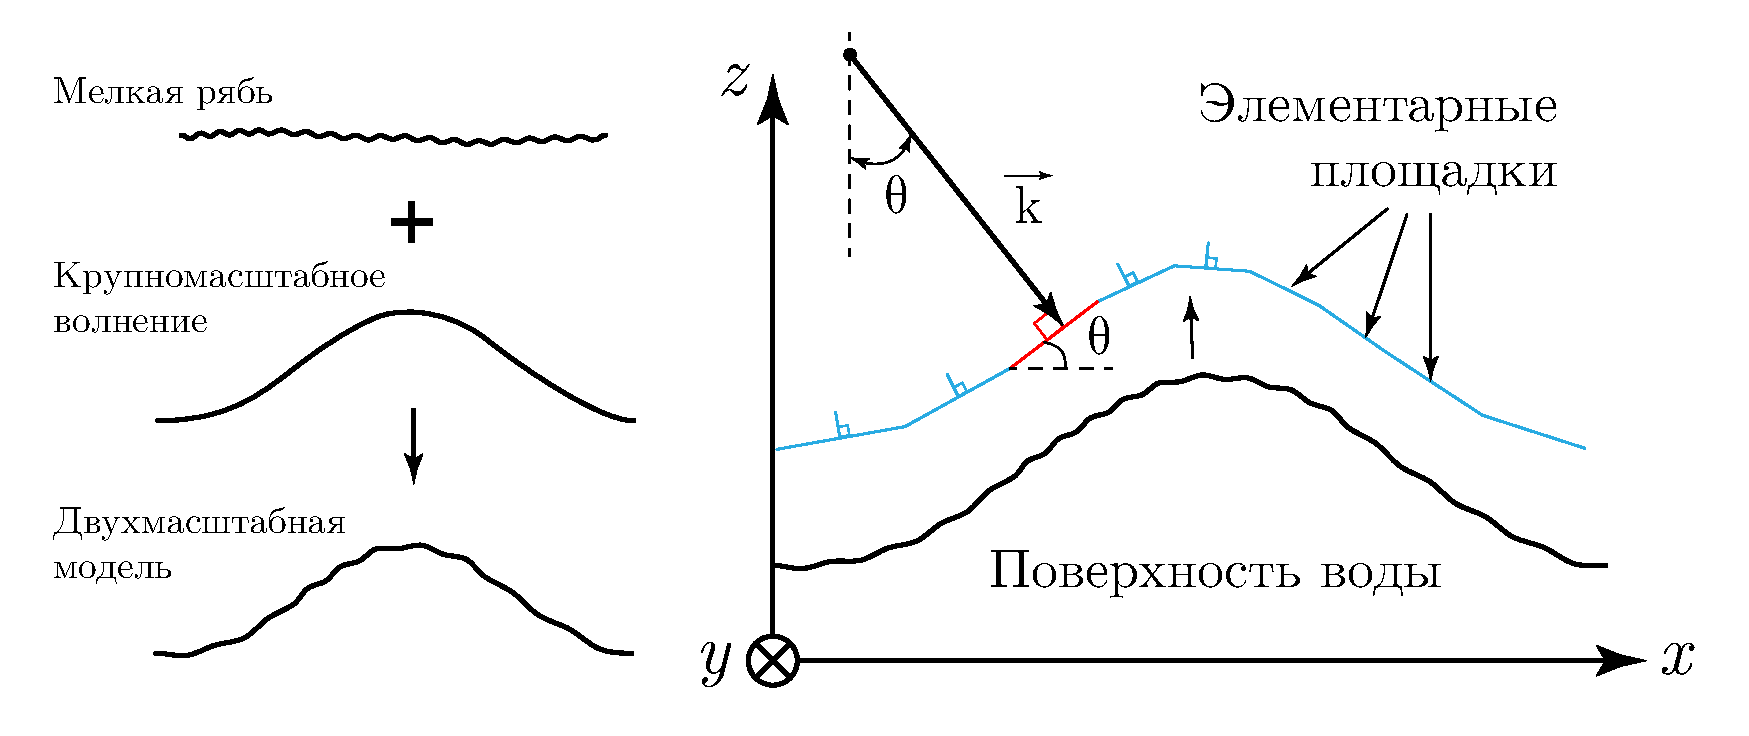
\includegraphics[width = .98\linewidth]{img/quazz.pdf}
  \caption{}
  \label{fig:2}
\end{figure}

Пусть морская поверхность описывается функцией $\zeta(x,y)$, и известна двумерная плотность распределения уклонов
морской поверхности $P_w(\zeta_x,\zeta_y)$. Для морской поверхности зависимость сечения рассеяния от угла падения
пропорциональна плотности распределения зеркальных площадок, которая равна
$P(\tan \theta, 0)$  \cite{bassfuks}:
\begin{equation}
  \sigma^0 = A (\cos \theta)^{-4} \cdot P_w(\tan \theta,0),
  \label{eq:3}
\end{equation}
где $\theta$ - угол отклонения от нормали (А – эффективный коэффициент отражения, на величину которого влияет наличие
ряби). Для воды такая $P_w(\zeta_x,\zeta_y)$ имеет вид распределения, близкого к нормальному \cite{masha}:
\begin{equation}
  P_w(\tan \theta) = \frac{1}{ 2 \pi \sigma_x \sigma_y } \cdot \exp (- \frac{\tan^2\theta}{2 \sigma^2_x})
  \label{eq:4}
\end{equation}
где $\sigma_{x,y}$ - дисперсии уклонов морской поверхности относительно осей $Ox$, $Oy$ соответственно. Они зависят, в
частности, от скорости ветра.

\section{Детектирование льда}
Для разработки метода детектирования льда, необходимо понять, чем ледяной покров отличается от водной поверхности по
данным двухчастотного радиолокатора. На рис. \ref{fig:3} приведены изображения Охотского моря за 27 декабря 2016
года в оптическом диапазоне, а также трек спутниковых данных Ku-диапазона радара DPR за тот же день.

\begin{figure}[h!]
  \centering
  \begin{minipage}{.49\linewidth}
    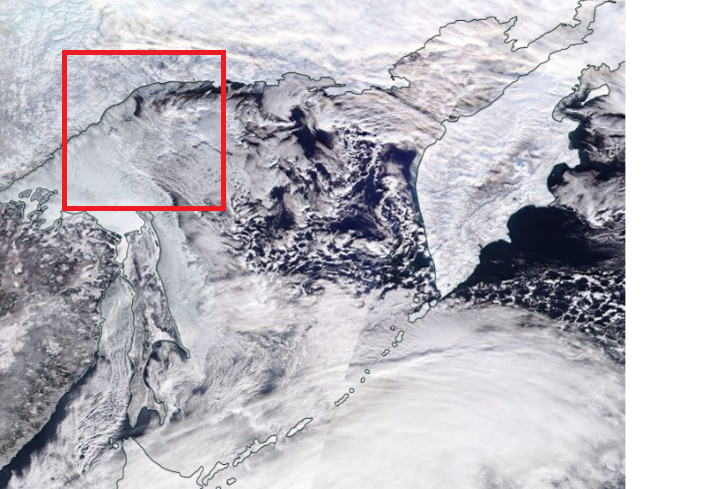
\includegraphics[width = \linewidth]{pic1.png}
  \end{minipage}
  \begin{minipage}{.49\linewidth}
    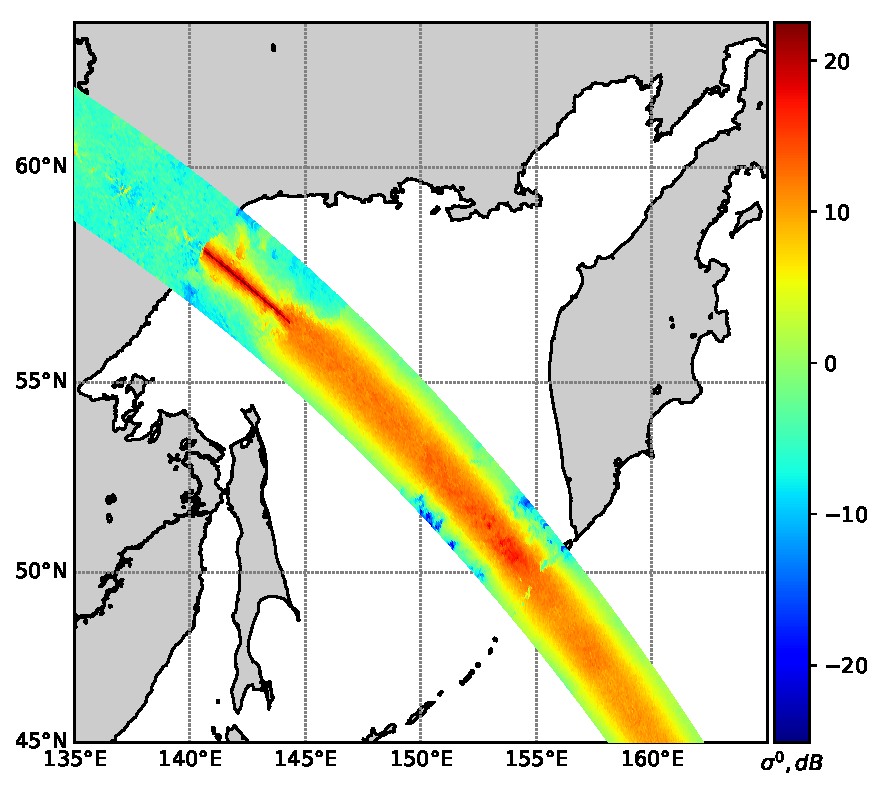
\includegraphics[width = \linewidth]{plot.pdf}
  \end{minipage}
  \caption{27.12.2016. Слева - оптическое изображение, справа - трек Ku-диапазона DPR (цветом обозначена $\sigma^0$ в дБ).}
  \label{fig:3}
\end{figure}

В области, обведенной красной рамкой (на снимке рис. \ref{fig:3}), присутствует ледяной покров. Через эту область также
проходит спутниковый трек, и наблюдаются характерные отличия в данных для обасти, покрытой льдом. Если рассматривать
поперечные
разрезы трека, т.е. угловую зависимость величины $\sigma^0(\theta)$, то мы получим картину на рис. \ref{fig:4} (слева), где
разные кривые соответствуют двум разным местам поперечного разреза, отмеченные на треке как две прямые линии
соответствующего цвета (черный - лед, красный - вода).

\begin{figure}[h!]
  \centering
  \begin{minipage}{.49\linewidth}
    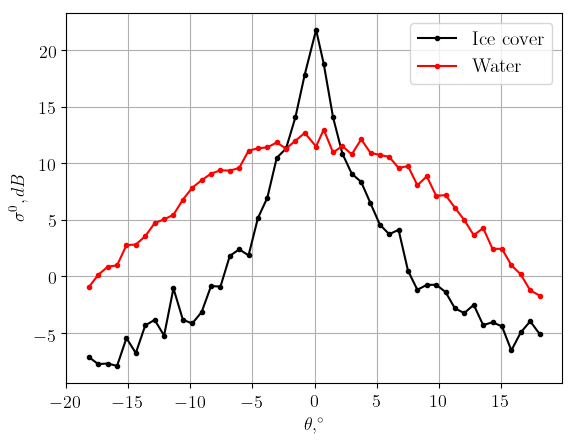
\includegraphics[width = \linewidth]{ice_cuts.png}
  \end{minipage}
  \begin{minipage}{.49\linewidth}
    \includegraphics[width = \linewidth]{plot_zoomed.pdf}
  \end{minipage}
  \caption{Слева - зависимости $\sigma^0(\theta)$ для поверхности льда (черный) и воды (красный), справа - трек Ku-диапазона, с отмеченными местами разрезов. }
  \label{fig:4}
\end{figure}

Как видно из рис. \ref{fig:4}, наблюдается существенная разница между зависимостями для поверхности льда и воды. Лед, по
отношению к воде, имеет б\'{о}льшие значения сигнала при малых углах падения и меньшие значения при больших углах, в то время как вода
имеет достаточно плавное распределение. Такую зависимость для льда можно объяснить в рамках
квазизеркального приближения. Так как лед - это достаточно гладкая поверхность, то при малых углах падения количество
перпендикулярных площадок намного больше, чем у воды, на которой постоянно присутствуют волнения. Следствием из этого
является большая отраженная энергия, а значит, и большее значение $\sigma^0$. 

При увеличении угла отклонения, количество зеркальных площадок на поверхности льда быстро спадает, и характер отражения сигнала
сменяется с квазизеркального на диффузный. При этом также быстро спадает количество отраженной энергии и велична УЭПР,
поэтому наблюдается такое резкое спаданение сигнала.

При анализе большого количества разрезов для ледяного покрова, все  угловые зависимости имели выделенный пик при нулевом
угле падения. Этот факт было решено использовать, как метод отличия ледяной поверхности от водной. В частности, для
того, чтобы определить, насколько выделенный пик имеет распределение, используется коэффициент эксцесса $\gamma_2$:
\begin{equation}
  \gamma_2 = \frac{\mu_4}{\sigma^4} -3,
  \label{eq:5}
\end{equation}
где $\mu_4$ - четвертый центральный момент, а $\sigma^2 = \mu_2$ - дисперсия. Для случайной величнины $x$ с известной плотностью вероятности $f(x)$, k-й
центральный момент это:
\begin{equation}
  \mu_k = \int \limits_{-\infty}^{\infty}(\overline{x}-x)^k f(x) dx,
  \label{eq:6}
\end{equation} 
где $\overline{x}$ - среднее значение величины $x$:
\begin{equation}
  \overline{x} = \int \limits_{-\infty}^{\infty}x f(x) dx.
  \label{eq:7}
\end{equation}

 

Разработка велась на языке программирования Python и его библиотеках. Как было описано ранее, в работе использовались
данные радиолокатора DPR, которые находятся в свободном доступе, и могут
быть предоставленны по запросу с \cite{data} в формате HDF5. Структура данных приведена на рис. \ref{fig:5}.

\begin{figure}[h!]
  \centering
  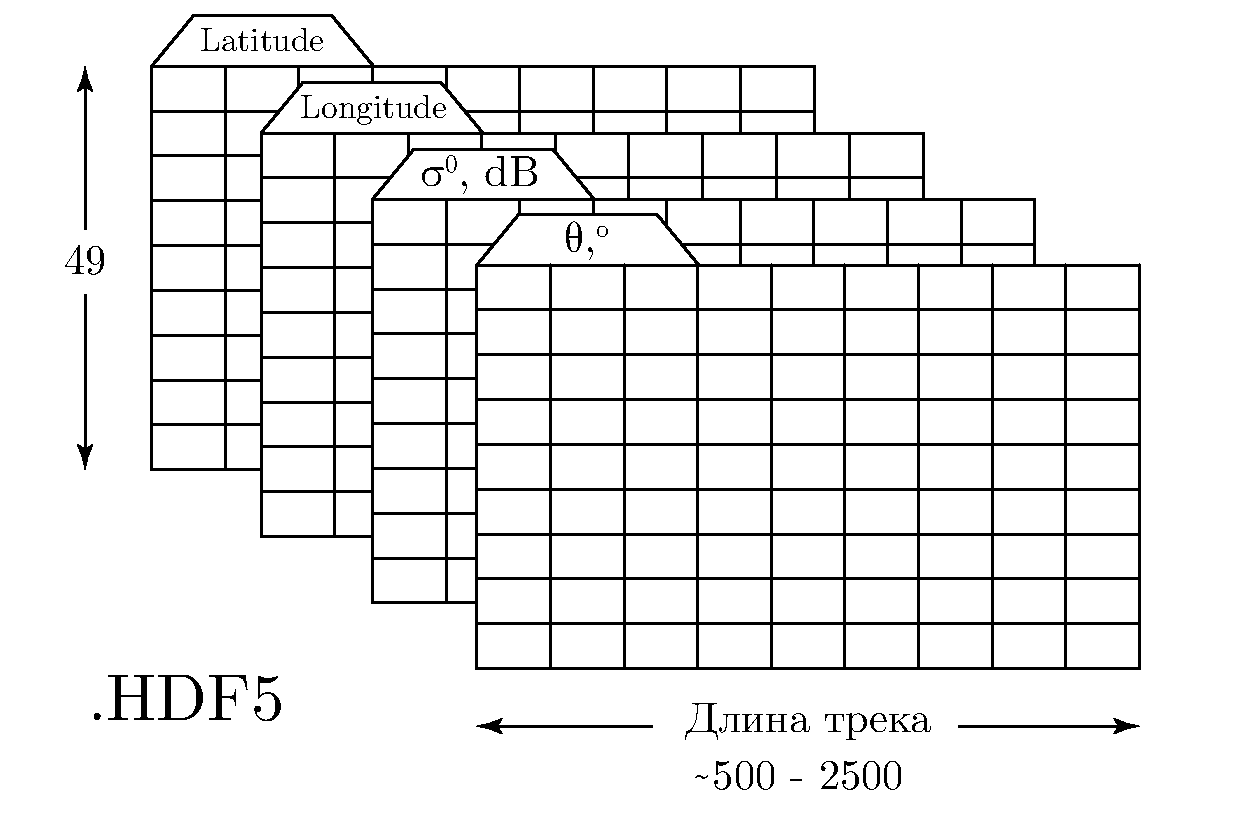
\includegraphics[width = 0.55\linewidth]{img/struct.pdf}
  \caption{Структура данных - набор массивов с данными}
  \label{fig:5}
\end{figure}

В файле .HDF5 содержатся массивы данных для координат - долгот\'{ы} и широт\'{ы}, угла падения, и значение $\sigma^0_{dB}$ в
дБ. 

\subsection{Методы валидации}

Для валидации произведенного детектирования использовались размеченные карты НИЦ «Планета» в виде полигонов областей и информацию об их содержании
- тип, возраст, сплоченость льда и др.. Зная координаты точки, ее значение $\sigma^0$ и угла падения, а также полигона,
которому она принадлежит, существующие данные можно разметить для валидации после работы алгоритма. 

Также для валидации использовались данные с радиометра (GMI), расположенного на том же спутнике, что упрощает нахождение
информации за конкретную дату, т.к. приборы установленны на одном спутнике. Стоит отметить, что данные радиометра имеют
большую точность в плане моментального снимка, в то время как карты, предоставленные НИЦ «Планета» представляют собой
результат накопления за 3х-4х-дневный период. Однако данные радиометра нужно предварительно обработать, и они не
обладают таким подробным описанием.

Имея размеченные треки, мы можем сравнить их с данными радиометра, расположенного на том же спутнике, а также с
картами «Планета».


\subsection{Коэффициент эксцесса}

Коэфиициента эксцесса $\gamma_2$ рассчитывается для плотности распределения зеркальных площадок $P(\tan \theta)$. При этом: 
\begin{equation}
  \sigma^0 = A \cos^{-4}(\theta) \cdot P(\tan \theta)
  \label{eq:8}
\end{equation}
Учитывая, что данные имеют значение для $\sigma^0_{dB}$ в дБ, то чтобы получить значение $P(\tan \theta)$ необходимо сделать
соответствующие преобразования:
\begin{equation}
  P(\tan \theta) =  \frac{\sigma^0 \cos^4(\theta)}{A},~ \sigma^0 = 10^{\frac{\sigma^0_{dB}}{10}}
  \label{eq:9}
\end{equation}

Для рассчета $\gamma_2$ необходимо рассчитать 2-й и 4-й центральные моменты для величины $\tan \theta$ и плотности $P(\tan \theta)$:
\begin{equation}
  \mu_k = \int \limits_{-\infty}^{\infty}(\overline{\tan \theta}-\tan \theta)^k P(\tan \theta) d(\tan \theta)
  \label{eq:10}
\end{equation} 
или в дискретном случае для $N = 49$ точек:
\begin{equation}
  \mu_k = \sum \limits_{n = 1}^{N} (\overline{\tan\theta} - \tan \theta_n)^k ~P(\tan \theta_n) \Delta(\tan \theta_n)
  \label{eq:11}
\end{equation} 
\begin{equation}
  \mu_k = \sum \limits_{n = 1}^{N} (\overline{\tan\theta} - \tan \theta_n)^k~ \frac{\sigma^0_n \cos^4(\theta_n)}{A} \Delta(\tan \theta_n)
  \label{eq:12}
\end{equation}
Для рассчета коэффициента $A$ воспользуемся нормирокой плотности распределения $P(\tan \theta)$:
\begin{equation}
  \int \limits_{-\infty}^{\infty} f(x)dx = 1 \Rightarrow \int \limits_{-\infty}^{\infty} P(\tan \theta) d(\tan \theta) = 1
  \label{eq:13}
\end{equation}
От бесконечных пределов мы можем перейти к области интегрирования, ограниченной массивами данных - максимальным и
минимальным углом отклонения, и свести к дискретному виду:
\begin{equation}
  \sum \limits_{n = 1}^{N} P(\tan \theta_n) \Delta(\tan \theta_n) = 1
  \label{eq:14}
\end{equation}
Подставляя в \eqref{eq:14} выражение \eqref{eq:9} получим:
\begin{equation}
  \sum \limits_{n = 1}^{N} \frac{\sigma^0_n \cos^4(\theta_n)}{A} \Delta(\tan \theta_n) = 1
  \label{eq:15}
\end{equation}
\begin{equation}
  A = \sum \limits_{n = 1}^{N} S^0(\theta_n) \Delta(\tan \theta_n),
  \label{eq:16}
\end{equation}
где $S^0(\theta_n) = \sigma^0_n \cos^4(\theta_n)$. Подставляя \eqref{eq:16} в \eqref{eq:12} для $\mu_k$ получим:
\begin{equation}
  \mu_k = \frac{\sum \limits_{n = 1}^{N} (\overline{\tan\theta} - \tan \theta_n)^k~ S^0(\theta_n) \Delta(\tan \theta_n)}{\sum \limits_{n = 1}^{N} S^0(\theta_n) \Delta(\tan \theta_n)}
  \label{eq:17}
\end{equation}
Ввиду дискретности измерений, величина $\Delta(\tan \theta_n)$ для всех измерений одинакова, и ее можно сократить как
общий множитель у верхней и нижней дроби. Среднее значение $\overline{\tan\theta}$ можно найти аналогично, из
определения среднего и нормировки плотности вероятности:
\begin{equation}
  \overline{\tan\theta} = \frac{\sum \limits_{n = 1}^{N} \tan \theta_n S^0(\theta_n) }{\sum \limits_{n = 1}^{N} S^0(\theta_n)}
  \label{eq:18}
\end{equation}
В итоге, для $\mu_k$ получим:
\begin{equation}
  \mu_k = \frac{\sum \limits_{n = 1}^{N} (\frac{\sum \limits_{n = 1}^{N} \tan \theta_n S^0(\theta_n) }{\sum \limits_{n = 1}^{N} S^0(\theta_n)} - \tan \theta_n)^k~ S^0(\theta_n)}{\sum \limits_{n = 1}^{N} S^0(\theta_n) }
  \label{eq:19}
\end{equation}
Рассчитывая значения $\mu_4$, $\mu_2$ и $\gamma_2$ для каждого поперечного разреза, сотсавляется массив из этих значений для
каждого трека. Пример результата рассчетов для данных на рис. \ref{fig:3} приведен на рис. \ref{fig:6}.

\begin{figure}[h!]
  \centering
  \begin{minipage}{0.50\linewidth}
    \centering
    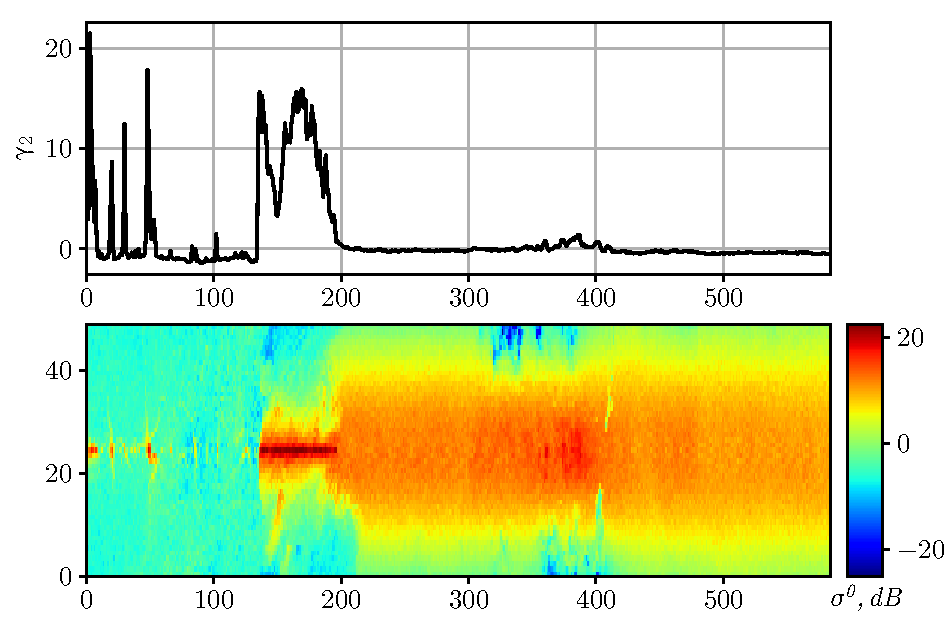
\includegraphics[width = \linewidth]{kurt.pdf}
    \caption{Сверху - коэффициент эксцесса $\gamma_2$ в зависимости от продольного номера разреза, снизу - трек данных}
    \label{fig:6}
  \end{minipage}
  \begin{minipage}{0.40\linewidth}
    \centering
    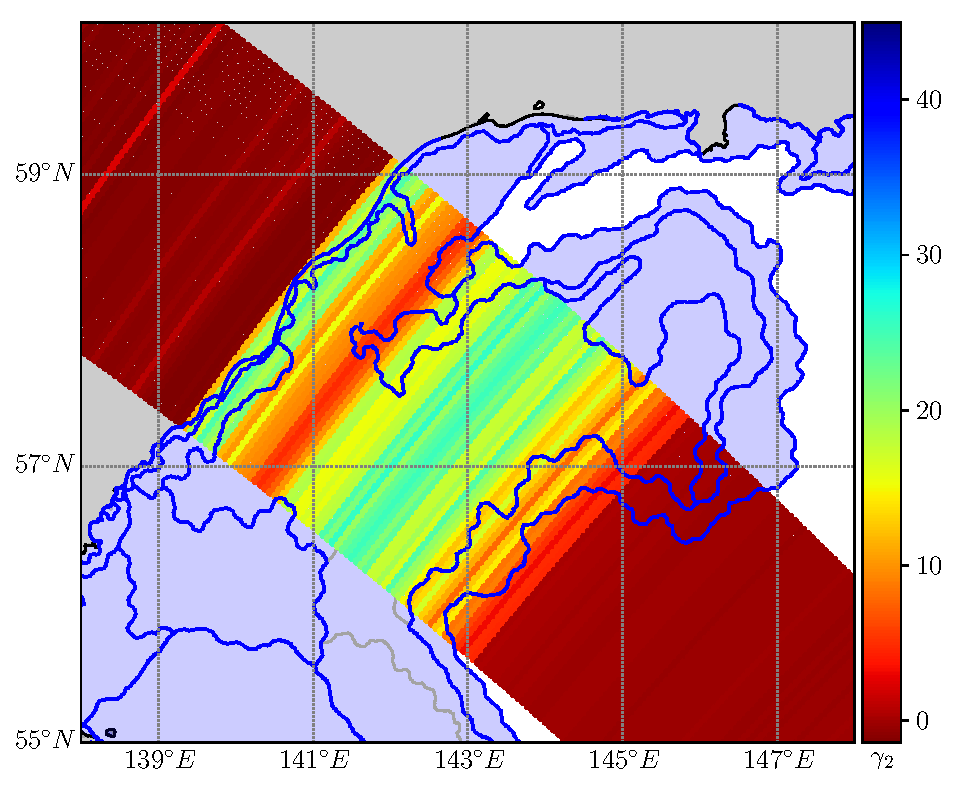
\includegraphics[width = \linewidth]{kurt2.pdf}
    \caption{Трек значений $\gamma_2$, наложенный на карту с разметкой ледяного покрова.}
    \label{fig:7}
  \end{minipage}
\end{figure}


Как видно из рис. \ref{fig:6}, коэффициент эксцесса для воды (область справа от номера 200) практически равен нулю, как
и должно быть для нормального распределения. В области номеров [0,130], географически находится
земля, ее можно убрать из рассмотрения и не обрабатывать. В области номеров [130,200] находится ледяной покров, и на  рис. \ref{fig:6}
видно, что для этой области коэффициент эксцесса значительно больше нуля, что позволяет численно отличить ледяную поверхность.

Однако рассчет коэффициента эксцесса дает очень грубое приближение о местонахождении льда. При таком рассчете,
используется вся ширина поперечного разреза, которая аналогична 245 км на поверхности Земли, и маркировка идет по
таким полосам. Визуально это представлено ни рис. \ref{fig:7}, где изначальный трек данных сохраняет ширину, но цветом
характеризуется не $\sigma^0$, а коэффициент эксцесса $\gamma_2$. Ледяной покров обозначен светло-синим цветом заполнения и
границами синего цвета. Там, где значения $\gamma_2$ высокие - порядка 15 - 20, с высокой вероятностью находится лед. В
остальных областях, где $\gamma_2$ меньше 15, возможны различные ситуации, и по такой оценке нельзя точно сказать, как
расположены поверхности воды и льда на данном разрезе. 



\subsection{Детектирование границ}
Один из способов уточнить изначальное приближение, полученное по коэффициенту эксцесса $\gamma_2$, это найти границы ледяного покрова.
Для определения границ необходимо детектировать скачки сигнала - $\sigma^0$. Рассмотрим зависимости УЭПР от продольной
координаты. Продольные срезы вдоль трека для разных углов падения приведены на рис. \ref{fig:8}.

\begin{figure}[h!]
  \centering
  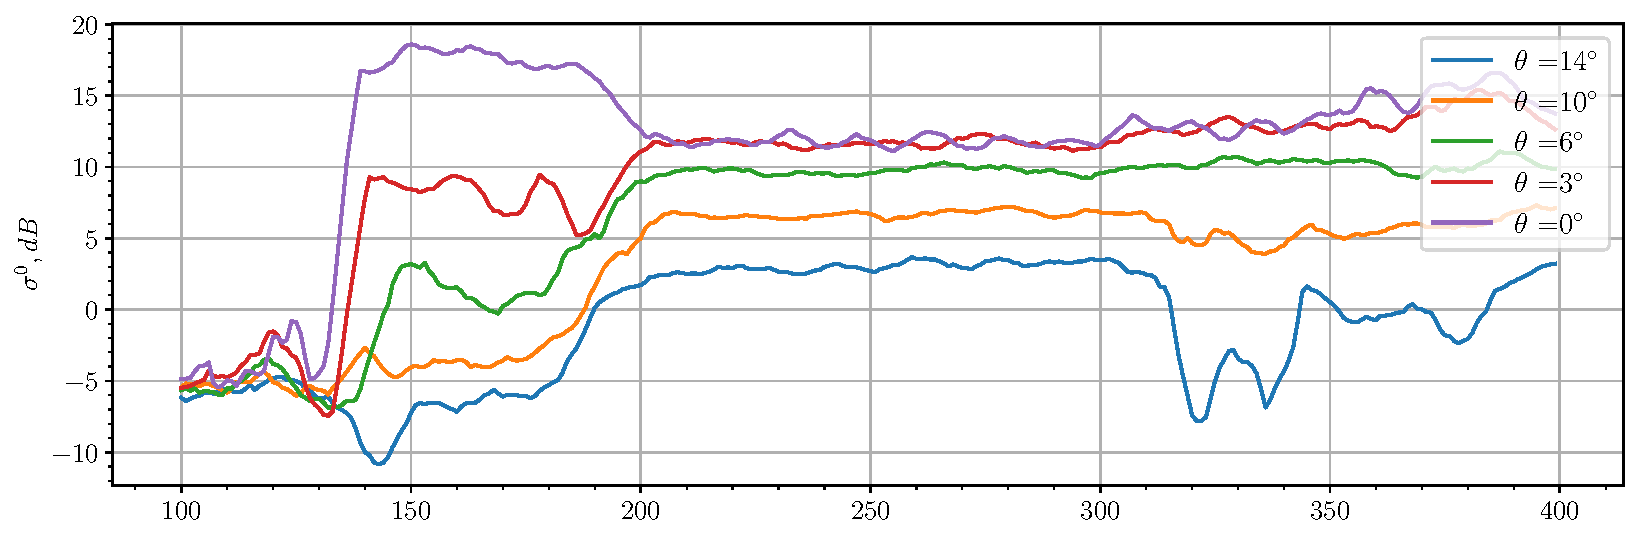
\includegraphics[width = 0.7\linewidth]{long.pdf}
  \caption{Продольные разрезы вдоль трека данных (см. рис. \ref{fig:6}) для различных углов падения.}
  \label{fig:8}
\end{figure}


Для выявления местонахождения скачка использовался алгоритм Джона Кэнни \cite{canny} для одномерного случая. Метод
заключается в произведении двух сверток - сигнала $G(x)$ и функции-детектора $f(x)$, результат которых здесь обозначен
как $S(x')$ ($x,x'$  - продольная координата). В качестве функции-детектора $f(x)$ используется производная
от Гауссового распределения \eqref{eq:fx}.  Локальные максимумы функции $S(x')$,
соответствуют скачкам сигнала, или в нашем случае, переходам
между различающимися по характеру рассеивания поверхностями. Например, на рис. \ref{fig:9} первый максимум отвечает за переход
земля-лед, а второй, слабее – за переход лед-вода. 

\begin{equation}
  S(x') = \frac{\left|\int \limits_{-W}^{+W} G(x'-x) f(x) d x\right|}{n_{0} \sqrt{\int \limits_{-W}^{+W} f^{2}(x) d x}} \frac{\left|\int \limits_{-W}^{+W} G^{\prime}(x'-x) f^{\prime}(x) d x\right|}{\sqrt{\int \limits_{-W}^{+W} f^{\prime 2}(x) d x}}
  \label{eq:S}
\end{equation}

\begin{equation}
  f(x) = -x\cdot \exp(-\frac{x^2}{2\sigma^2_g})
  \label{eq:fx}
\end{equation}


\begin{figure}[h!]
  \centering
  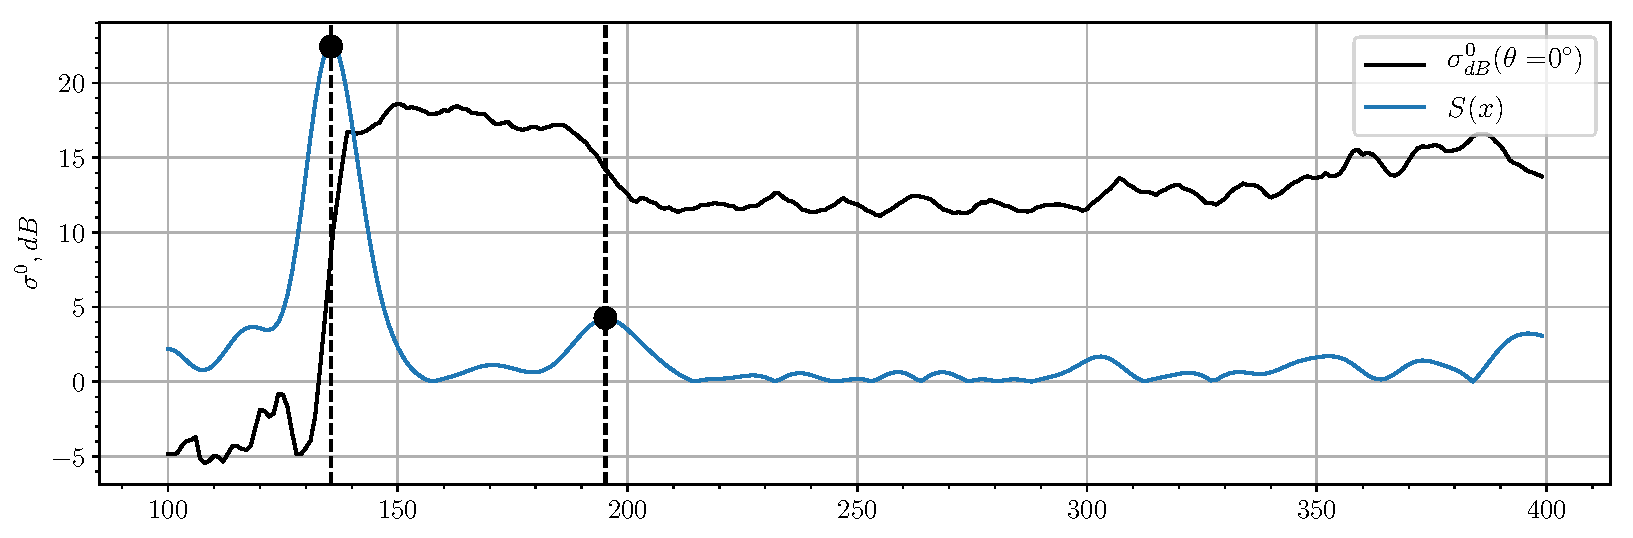
\includegraphics[width = 0.7\linewidth]{long2.pdf}
  \caption{Продольный разрез для $\theta = 0^{\circ}$ и результат работы фильтра $S(x)$}
  \label{fig:9}
\end{figure}

На чувствительность алгоритма влияет вид функции-детектора - ширина гауссового распределения $\sigma_g$. При этом
функция-детектор должна полностью убиралаться в окно свертки $[-W,+W]$. При этом фильтр не может быть слишком чувствительным. Чем уже
функция-детектор $f(x)$, тем на меньшие скачки она реагирует, из-за чего функция $S(x')$ может стать очень шумной. В
работе был выбран оптимальный вариант соотношения ширины окна свертки и ширины функции, для наилучшего
детектирования ( $\sigma_g = 1.1, W = 5$. Стоит отметить, что при значениях $W>3\cdot \sigma_g$, вклад на крыльях
функции-детектора уже не существенен из-за близости значений к нулю. ). 

Оописанный выше метод обнаружения границ применялся к каждому продольному разрезу, откуда находились локальные
максимумы функции $S(x')$, соответствующие местам скачков сигнала, или, в нашем случае, границам отражающих
поверхностей. Пример полученной карты границ приведен на рис. \ref{fig:10}.

\begin{figure}[h!]
  \centering
  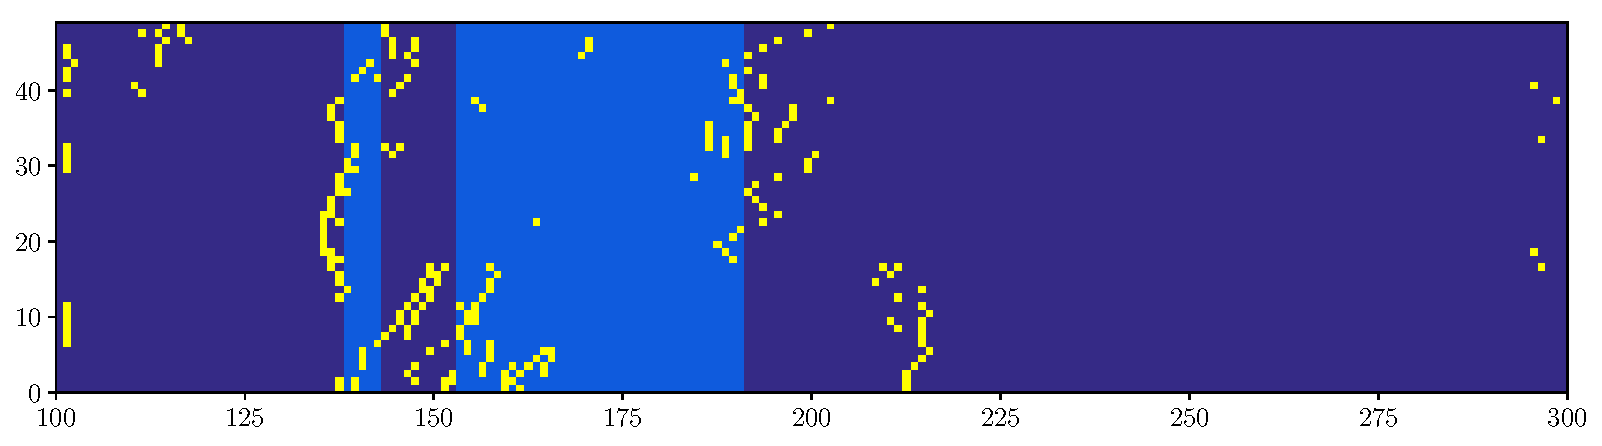
\includegraphics[width = 0.7\linewidth]{f1.pdf}
  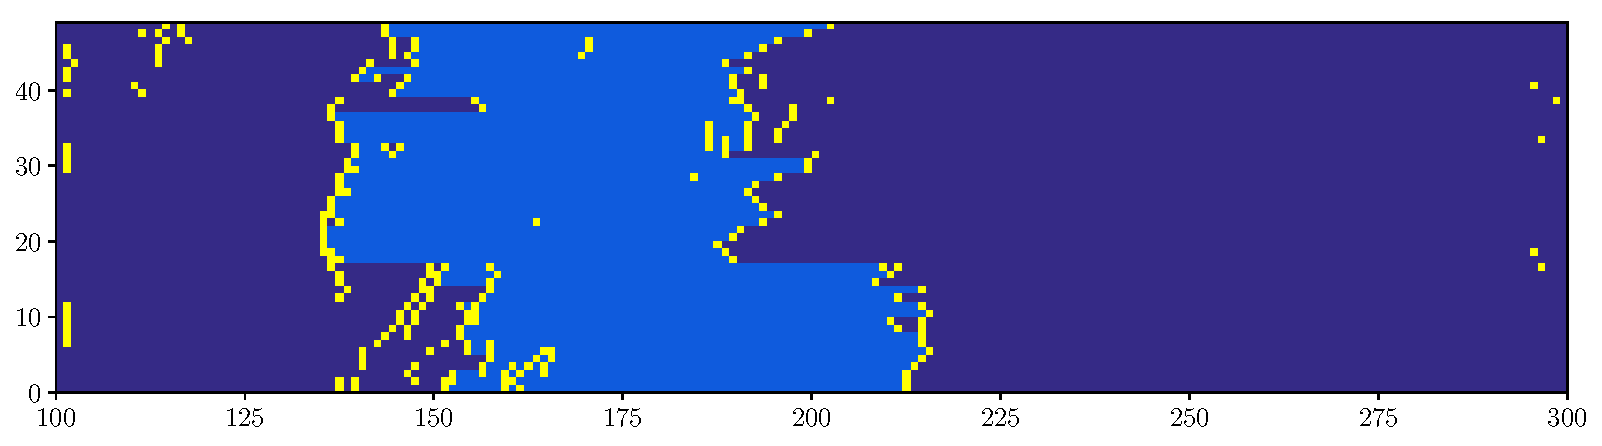
\includegraphics[width = 0.7\linewidth]{f2.pdf}
  \caption{Карта границ и льда для массива данных на рис. \ref{fig:6}.}
  \label{fig:10}
\end{figure}

Совмещая карту границ и карту расположения льда для получения более точной картины, мы можем заполнить ограниченные
области, в соответствии с их содержанием. Если в ограниченной области - области между двумя границами, находится
преимущественно (например, 60\%) лед, то происходит заполнение всей
области льдом. В противоположном случае, при нахождении в области недостаточного количества льда - т.е. лед был
обнаружен ошибочно из-за грубого первоначального приближения, ограниченная область заполняется пустым флагом.
Примеры результатов работы алгоритма приведены на рис. \ref{fig:11}(а также сравнение с данными радиометра в приложении на рис. \ref{fig:11}).

\begin{figure}[h!]
  \centering
  \begin{minipage}{0.48\linewidth}
    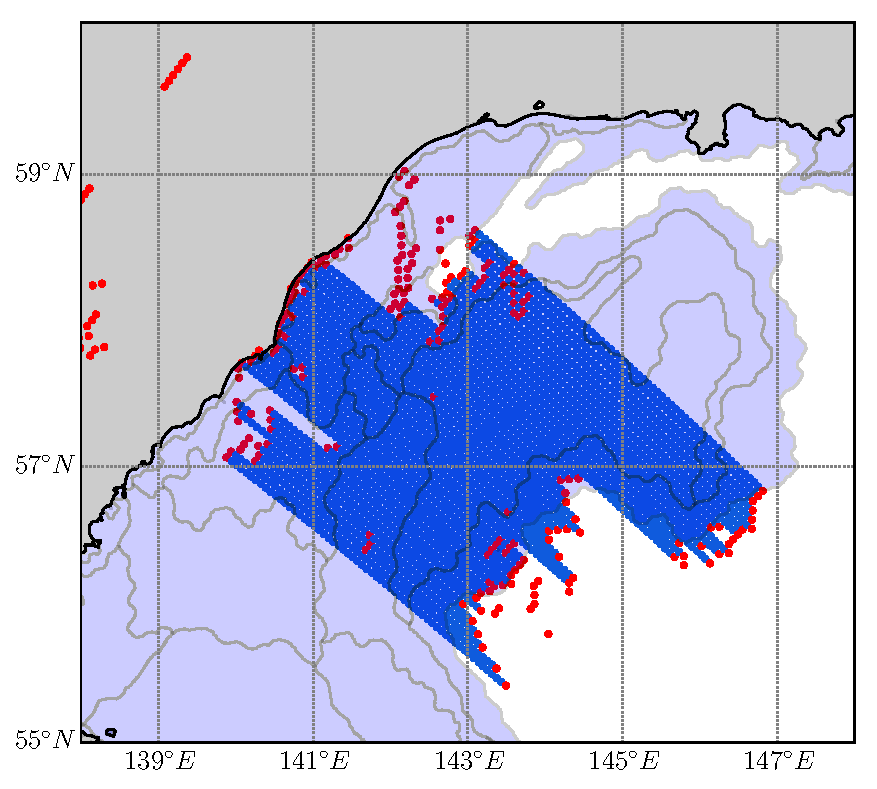
\includegraphics[width = \linewidth]{map1.pdf}
    \caption{Карта льда, наложенная на полигоны карт НИЦ Планета}
    \label{fig:11}
  \end{minipage}
  \begin{minipage}{0.51\linewidth}
    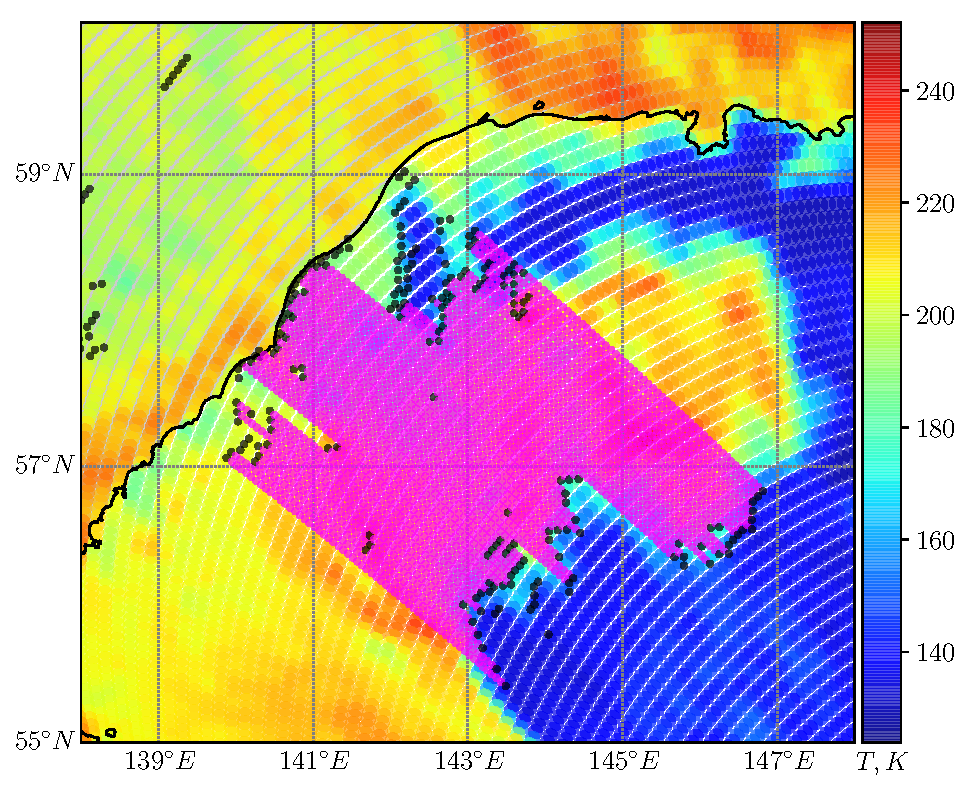
\includegraphics[width = \linewidth]{map2.pdf}
    \caption{Карта льда, наложенная на данные радиометра(36.6 ГГц H-Pol)}
    \label{fig:12}
  \end{minipage}

\end{figure}

На рис. \ref{fig:11} и рис. \ref{fig:12} видно, что наблюдается совпадение между существующими картами, и картами, составленными
по данным DPR. При этом, сравнивая рис. \ref{fig:11} и рис. \ref{fig:12}, наблюдается б\'{о}льшее совпадение полученных
результатов с данными радиометра. Однако совпадение преимущественно в общих чертах, не все детали были захвачены. В основном,
пропуски происходят при попадании на срез нескольких типов поверхности. Все вышеописанные методы в таком случае работают на несколько порядков
хуже, или не работают вовсе. Чтобы детектировать лед в таких ситуациях, необходимо рассматривать каждую точку отдельно,
учитывая множество параметров.

\section{Заключение}

В результате нашей работы был разработан алгоритм, позволяющий детектировать расположение ледяного покрова на
поверхности моря, используя данные двухчастотного локатора DPR, расположенного на спутнике GPM. 

Алгоритм достаточно хорошо работает в случаях, когда на поверхности поперечного разреза находится один (или
преимущественно один) тип отражающей поверхности. Его работа не зависит от облачности (кроме от осадков, эти данные изначально не
рассматриваются), и позволяет определить ледяной покров в те дни, когда оптические изображения затянуты облаками. 

Из недостатков можно отметить неточную работу алгоритма при попадании на срез нескольких типов отражающей поверхности. В
таком случае расчет коэффициента эксцесса не имеет смысла из-за кусочного вида угловой зависимости. 

Одним из методов дальнейшего улучшения работы является использование второго диапазона частот, полоса которого была
расширена до аналогичной Ku - диапазону. Также, ввиду симметрии относительно угла отклонения, полосу трека можно
разделить пополам на две одинаковые, и считать коэффициент эксцесса для зеркально отраженного распределения. Также, при
наличии размеченных карт, становится возможным использование машинного обучения для решения задачи классификации, имея
различные параметры - величина сигнала, угол падения, время года, и т.д. 


\newpage
\addcontentsline{toc}{section}{Список литературы}
\begin{thebibliography}{99}
\bibitem{skof} Skofronick-Jackson, G., W.A. Petersen, W. Berg, C. Kidd,
E.F. Stocker, D.B. Kirschbaum, R. Kakar, S.A. Braun, G.J. Huffman, T. Iguchi, P.E. Kirstetter, C. Kummerow, R.
Meneghini, R. Oki, W.S. Olson, Y.N. Takayabu, K. Furukawa, and T. Wilheit, 2017: The Global Precipitation Measurement
(GPM) Mission for Science and Society. Bull. Amer. Meteor. Soc., 98, 1679–1695,
https://doi.org/10.1175/BAMS-D-15-00306.1 
\bibitem{chu} Chu, X., He, Y., \& Karaev, V. Y. (2012). Relationships between ku-band
radar backscatter and integrated wind and wave parameters at low incidence angles. IEEE Transactions on Geoscience and
Remote Sensing, 5, 4599–4609.
\bibitem {fre} Freilich, M., \& Vanhoff, B. (2003). The relationship between winds, surface roughness, and radar
backscatter at low incidence angles from trmm precipitation radar measurements. Journal of Atmospheric and Oceanic
Technology, 20, 549–562.
\bibitem{kar1} V. Karaev, M. Panfilova, Y. Titchenko, E. Meshkov, G. Balandina, Z. Andreeva, Monitoring of Inland Waters
by Dual-Frequency Precipitation Radar: First Results, IEEE Journal
of Selected Topics in Applied Earth Observations and Remote Sensing, 2018, PP. 1-9, 10.1109/JSTARS.2018.2874697
\bibitem{masha} M.A. Panfilova, V.Yu. Karaev, Jie Guo, Oil Slick Observation at Low Incidence Angles in Ku-Band, Journal of Geophysical Research,
Oceans, March 2018, pp. 1-13, doi.org/10.1002/2017JC013377
\bibitem{meln} Мельник Ю.А., С.Г. Зубкович. Радиолокационные методы исследования Земли. - Советское радио, 1980 - 7 с.
\bibitem{bassfuks} Басс Ф.Г., Фукс И.М. Рассеяние волн на статистически неровной поверхности. - Наука, 1972. - 200 с.
\bibitem{data} NASA STORM https://storm.pps.eosdis.nasa.gov/storm
\bibitem{land} Ландау Л.Д., Лифшиц Е.М. Теоретическая физика: т.5, Статистическая физика. - М.: Физматлит, 2005. - 616 с.
\bibitem{canny} J. Canny. A computational approach to edge detection (1986). IEEE Transactions on pattern analysis and machine
learning, 6, 679-698.
\end{thebibliography}

\newpage
\addcontentsline{toc}{section}{Приложение}
\section*{Приложение}

\begin{table}[h!]
  \centering
  \caption{Технические характеристики DPR}
  \vspace{10 pt}
  \begin{tabular}{l|l|l}
   Характеристика & Ku - диапазон & Ka - диапозон \\ \hline
   Частота & 13.6 ГГц & 35.5 ГГц \\ \hline
   Ширина полосы обзора & 245 км & 120 км \\\hline
   Вертикальное разрешение & 250 м & 250-500 м \\\hline
   Пространственное разрешение & 5 км & 5 км \\\hline
   Частота повторения импульса & 4.1 - 4.4 кГц & 4.1 - 4.4 кГц \\\hline
   Количество точек & 49 & 49 
   \end{tabular}
  
  \label{tab:1}
\end{table}

\begin{table}[h!]
  \centering
  \caption{Технические характеристики спутника GPM}
  \vspace{10 pt}
  \begin{tabular}{l|l}
   Высота полета: 407 км & Наклон орбиты: 65 $^{\circ}$\\ \hline
     Период орбиты: 93 м & Орбита: круговая \\ \hline
     Скорость полета: 7 км/с & Оборотов за сутки: $\approx$16
  \end{tabular}
  
  \label{tab:1}
\end{table}


\begin{figure}[h!]
  \centering
  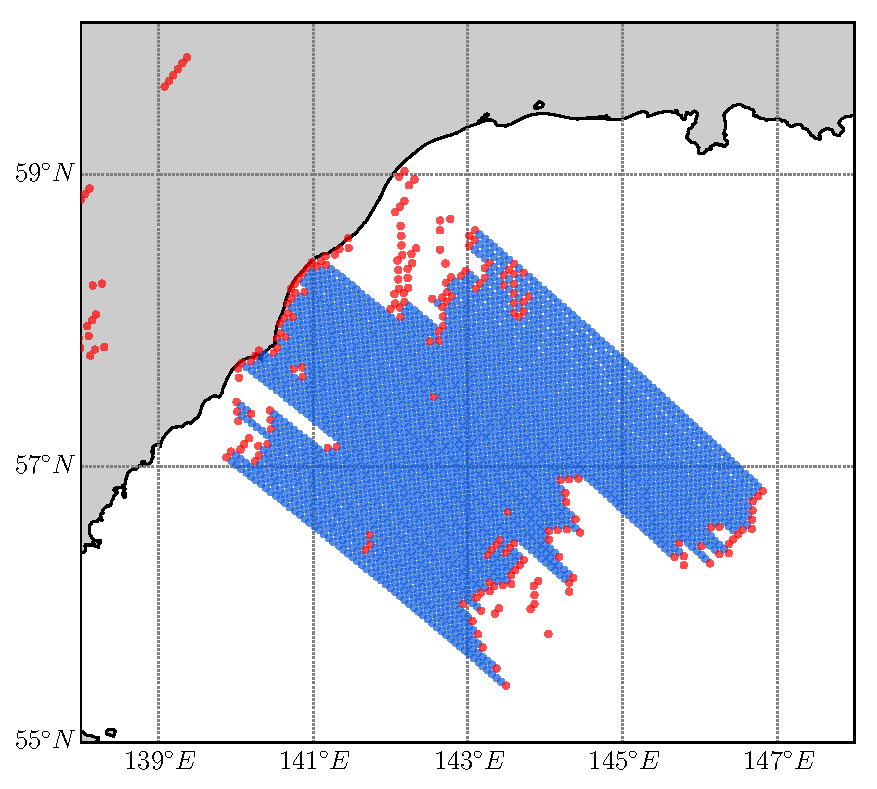
\includegraphics[width = .6\linewidth]{map4.pdf}
  \caption{Карта льда, составленная по данным DPR за 27.12.2016}
  \label{fig:15}
\end{figure}

\begin{figure}[h!]
  \centering
  \begin{minipage}{0.49\linewidth}
    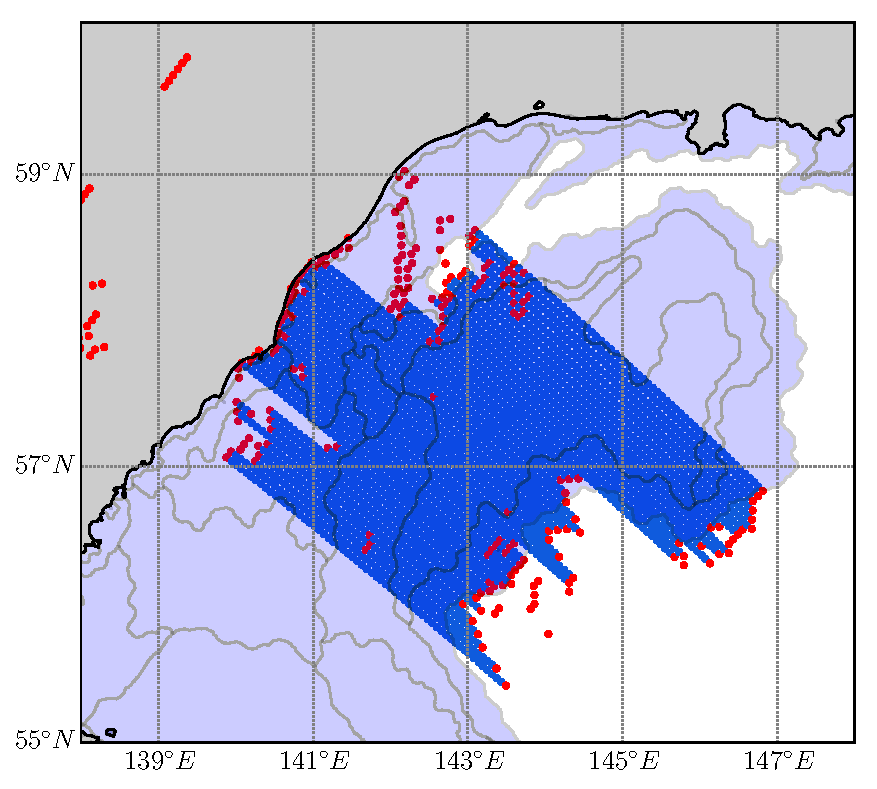
\includegraphics[width = \linewidth]{map1.pdf}
    \caption{Карта льда, наложенная на полигоны карт НИЦ Планета}
    \label{fig:13}
  \end{minipage}
  \begin{minipage}{0.49\linewidth}
    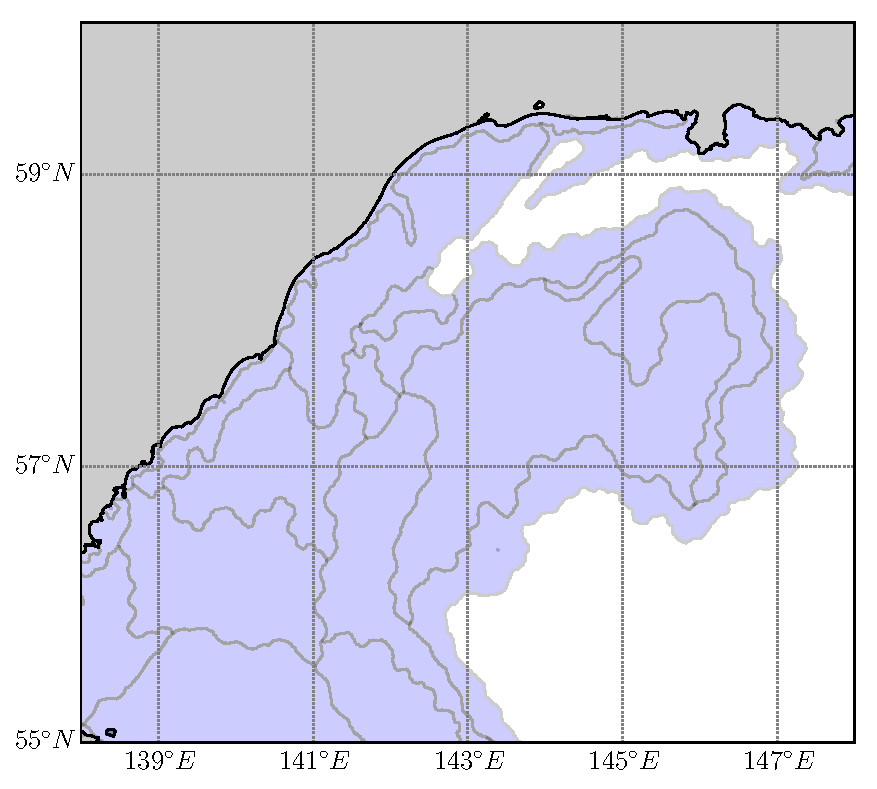
\includegraphics[width = \linewidth]{map11.pdf}
    \caption{Полигоны карт НИЦ Планета (несколько типов льда)}
    \label{fig:14}
  \end{minipage}

\end{figure}




\begin{figure}[h!]
  \centering
  
  \begin{minipage}{0.49\linewidth}
    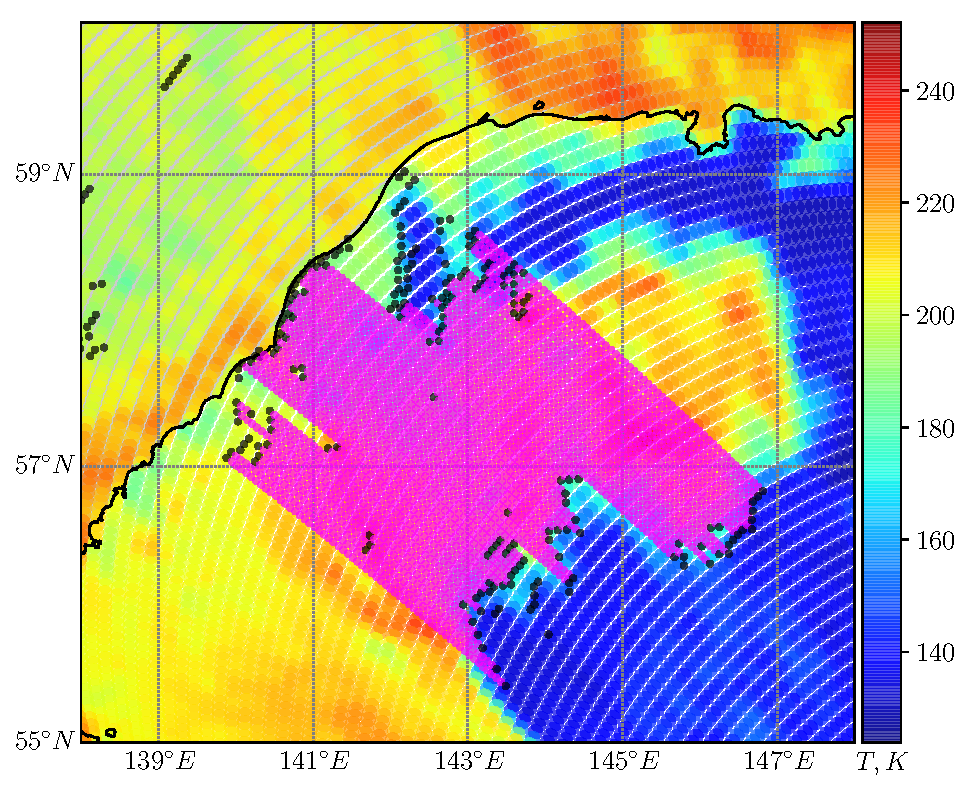
\includegraphics[width = \linewidth]{map2.pdf}
    \caption{Карта льда, наложенная на данные радиометра(36.6 ГГц H-Pol)}
    \label{fig:16}
  \end{minipage}
  \begin{minipage}{0.49\linewidth}
    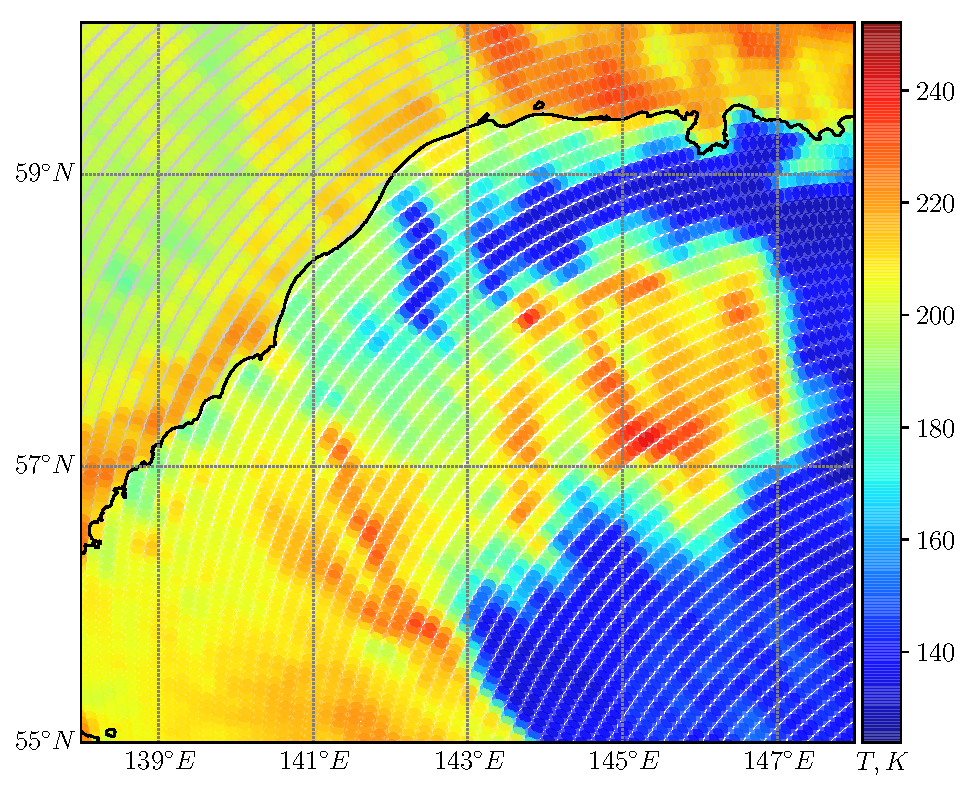
\includegraphics[width = \linewidth]{map21.pdf}
    \caption{Данные радиометра(36.6 ГГц H-Pol)}
    \label{fig:17}
  \end{minipage}

\end{figure}

\end{document}